\documentclass[b5paper]{ctexbook}
\author{Peterlits}
\title{高中物理}

\usepackage[colorlinks,linkcolor=black]{hyperref}
\usepackage{graphicx}
\usepackage{caption}
\usepackage{wrapfig}
\usepackage{amsmath}
\usepackage{footnote}
\usepackage{fancyhdr}
\usepackage{layout}
\usepackage{enumitem}[shortlabels]

\setlist{leftmargin=4em, itemsep=0.1em, parsep=0em, topsep=0.2em, 
			itemindent=0em, listparindent=0em, labelwidth=1em, labelsep=1em}

\newcommand{\mathline}{\ \_\_\_\_\_\_\ }
\newcommand{\mathc}{\hfill\mbox{(\mathline)}}
% nl:new line
\newcommand{\mathcnl}{\\\makebox[\linewidth][r]{(\mathline)}}
\renewcommand{\figurename}{图}
\newcommand{\emptypage}{
	\newpage
	\thispagestyle{empty}
	\phantom{this page should be empty}
	\newpage
}

\newenvironment{enumc}
	{\begin{enumerate}[label=(\arabic*), labelsep=0.5em, labelwidth= 1.5em]}
	{\end{enumerate}}

\setlength{\marginparwidth}{0pt}
\setlength{\oddsidemargin}{20pt}
\setlength{\evensidemargin}{-9pt}

\begin{document}
	% \layout
	\thispagestyle{empty}
	\maketitle

	\emptypage

	\pagenumbering{Roman}
	\tableofcontents

	\emptypage
	
	\pagenumbering{arabic}
	\mainmatter
   \chapter{机械运动与物理模型}
	\section{内容要求}
		根据\emph{普通高中物理课程标准(2017年版)},该节需要:

		\begin{itemize}
			\item 了解近代实验科学产生的背景,认识实验对物理学发展的推动作用。
			\item 经历质点模型的构建过程,了解质点的意义。
			\item 理解位移、速度和加速度。
			\item 通过实验,了解探究匀变速直线的特点。使用公式、图像描述匀变速直线运动,理解其规律。
			\item 通过实验,认识自由落体运动规律。
			\item 结合实验学史的相关内容,认识物理实验和科学推理在物理学研究中的作用。
		\end{itemize}

		而根据教学形式与传统形式不同(\emph{补课}),所以着重落在\emph{辅为主}的基本原则。%
		争取\emph{细、全、补、预}四个方面牢抓狠抓:
		\begin{verse}
			\emph{细},围绕考试大纲为主,不放过任何一个考点考型。\\
			\emph{全},注重框架化,辅导中把结构放在第一位。\\
			\emph{补},查漏补缺,是学习中最重要的一环。每个课时都有大量的联系,不仅可以加速掌握知识的速度,更能了解到学生的详细情况。\\
			\emph{预},在老师上课前提前预习。
		\end{verse}

		同时\emph{不仅要在课上下功夫,课下,在学做人、学做事之外,也不应该放下学业},祝同学在生活上做一个\emph{清醒、正直又有趣的人},在学业上做一个\emph{热爱智慧的人}。
	
	\section{正文}
		\subsection{质点\ 参考系和坐标系}
			\subsubsection*{质点}
				质点模型是高中提出的第一个理想模型\footnote{Q:什么是模型?什么是理想模型?怎么构建一个模型?}。
				
				描述物体运动的困难和麻烦有很多 ------ 运动物体各不相同,属性也各不相同\footnote{\ldots “如果物体都是只有质量,没有形状的一个点,那问题就简单了\ldots ”\ldots}。%
				为了描述运动过程,就必须要提炼出运动物体的共性,于是质点模型出现了。

				既然质点是为了描述运动状态的一种理想模型,什么物体可以视为质点呢\footnote{我想答案就在前一句话里。}?

			\subsubsection*{参考系}
				初中时已经学过参考物,而参考系和参考物本质上并无不同,只是参考系是一种更为科学的名字。

			\subsubsection*{坐标系}
				坐标系是数学知识在物理学科中的应用。

				坐标系的存在是为了确认做运动的物体的位置。为了定量描述物体的位置及位置的变化,需要在参考系上建立适当的坐标系\footnote{这是书上的一段原话,将第一节中的两个系的概念互相联系起来。(\emph{我觉得好棒的说})}。

			\subsubsection{例题}
				\paragraph{1}
					“一江春水向东流”说明了怎样的运动情况?那么“地球的公转”呢?“太阳东升西落”呢?
				\paragraph{2}
					一个人相对于一匀速运动的车厢欲把物体水平抛出,他观察到的现象是“物体做水平运动”吗?对于车厢外的人来说,他可能会观察到什么现象?\footnote{原题是:一人在车厢中把物体抛出,那种情况下,乘客在运动车厢里观察到是现象和在静止车厢里观察到的现象一样?(\emph{选项:车厢匀速直线行驶时;车厢减速时;车厢转弯时;车厢加速行驶时})}
				\paragraph{3}
					\begin{figure}[hbt]
						\centering
						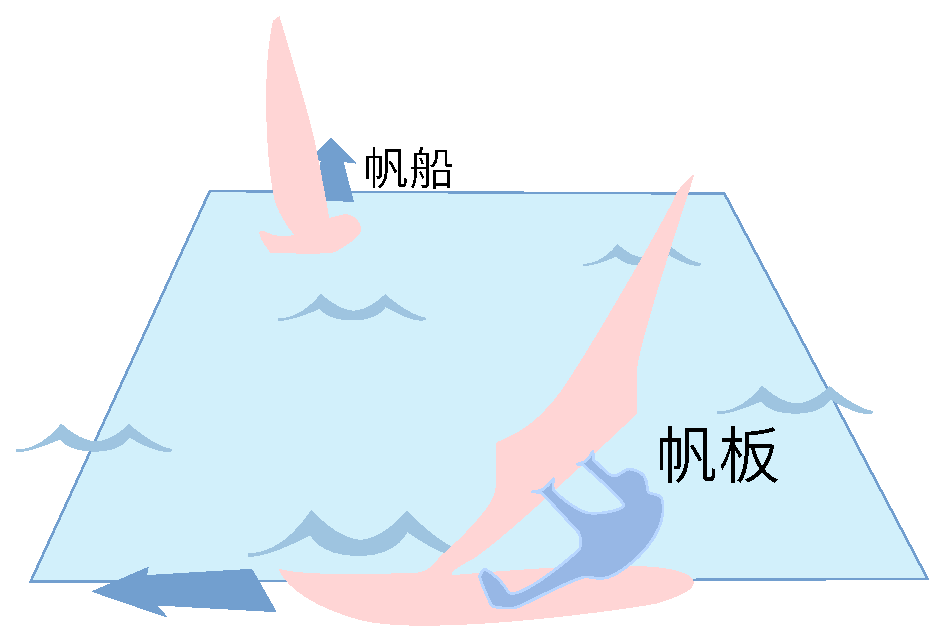
\includegraphics[scale=0.3]{PIC/001.eps}
						\caption{正在行驶的帆船和帆板}
						\label{Pic::正在行驶的帆船和帆板}
					\end{figure}
					见图\ref{Pic::正在行驶的帆船和帆板}\footnote{图真的好难画啊\ldots },帆板在海面上以速度$v$朝正西方向运动,帆船以速度$v$朝正北方向航行,以帆板为参照物,有\mathcnl\\
					A. 帆船朝正东方向航行,速度大小为$v$.\\
					B. 帆船朝正西方向航行,速度大小为$v$.\\
					C. 帆船朝南偏东$45^\circ$方向航行,速度大小为$\sqrt{2}v$.\\
					D. 帆船朝北偏东$45^\circ$方向航行,速度大小为$\sqrt{2}v$.\\
				\paragraph{4}
					下列说法正确的是\mathc\\
					A. 由于“辽宁舰”“高大威武”,故任何情况下都不能看成质点.\\
					B. 战斗机飞行员可以把正在甲板上用手势指挥的调度员看做一个质点.\\
					C. 在战斗机飞行训练中,研究战斗机的空中翻滚动作时,战斗机可以看做质点.\\
					D. 研究“辽宁舰”航母在大海中运动轨迹时,航母可以看做一个质点.\\
				\paragraph{5}(\emph{泰州中学高三学情检测})
					帆船即利用风力前行的船,帆船起源于荷兰,古代的荷兰,地势很低,所以开凿了很多运河,人们普遍使用小帆船运输或捕鱼,到了13世纪,威尼斯开始定期举办帆船运动比赛,当时比赛船还没有统一的规格和级别,1900年第2届奥运会开始将帆船运动列为比赛项目.帆船前进时,船员感觉岸上的树木向后移动,他所选择的参考系是\mathcnl\\
					A. 河水.\\
					B. 河岸.\\
					C. 帆船.\\
					D. 天空.\\
		\subsection{时间和位移}
			\subsubsection*{时间和时刻}
				什么是时间?什么是时刻?它们之间的概念有什么区别?
			\subsubsection*{路程和位移}
				什么是路程?什么是位移?它们之间的概念又有什么区别?\footnote{在这两个基础上的速度和速率呢?}
			\subsubsection{例题}
				\paragraph{1}
					\begin{wrapfigure}[10]{r}{5.5cm}
						\centering
						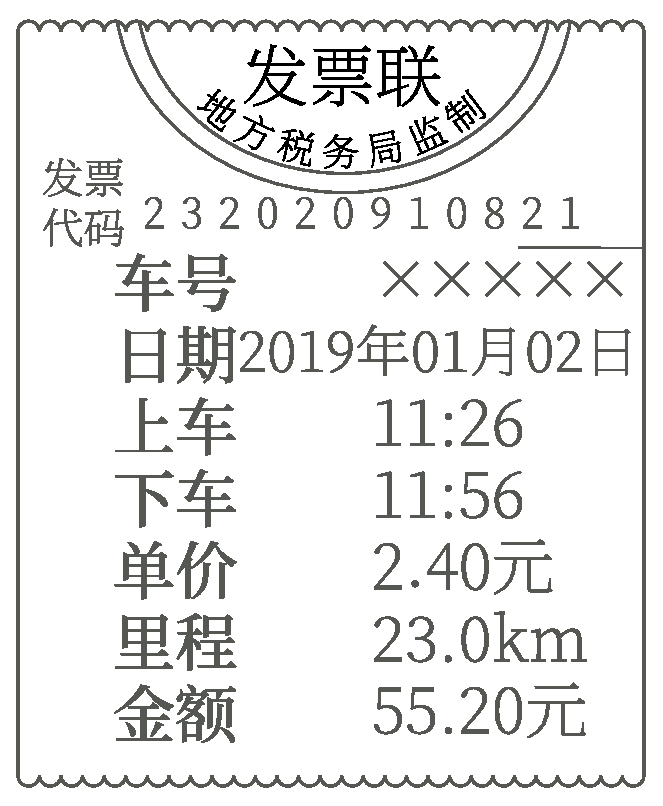
\includegraphics[scale=0.35]{PIC/002.eps}
						\caption{全程的发票}
						\label{Pic::全程的发票}
					\end{wrapfigure}
					(\emph{无锡市高三期初联考,多选})
					小明坐出租车到车站接人后返回出发地,
					司机打出全程的发票如图\ref{Pic::全程的发票}所示,由发票中的信息可知\mathc\\
					A. $11:26$是指时间间隔.\\
					B. 出租车的位移为$23.0 km$.\\
					C. 出租车的平均速度是$0$.\\
					D. 出租车的平均速度是$46 km/h$.\\
				\paragraph{2}\footnote{关于速度、加速度下一小节会讲到.}
					下列说法正确的是\mathc\\
					A. 高速公路路牌上显示“南京$100 km$”,表示该处距离南京的位移大小为100km.\\
					B. 博尔特比别的运动员起跑快,是因为他的加速度比别的运动员大.\\
					C. 磁悬浮列车运动得很快,我们说它的加速度很大.\\
					D. 马拉松运动员完成赛程,又跑回原来出发的体育场,我们说他的位移很大.\\
				\paragraph{3}(\emph{句容高级中学高三月考})
					建筑工地上的起重机把一筐砖先竖直向上提升$40 m$,然后沿半径为$30 m$的圆弧水平转过$60^\circ$,此过程中砖块的路程和位移大小为\mathc\\
					A. 路程大于$70 m$,位移为$50m$.\\
					B. 路程和位移都大于$50 m$.\\
					C. 路程为$70 m$,位移为$50 m$.\\
					D. 路程和位移都是$70 m$.\\
		\subsection{运动快慢的描述 ----- 速度}
			\subsubsection*{速度与速率}
				在上一小节中提到过,速度是以位移和时间\footnote{它们前两个相对应的标量单位又是什么呢?时间对应时间维度的一根线的话,对应一个点的物理量又是什么呢?}为基础而引出的,所以,速度和位移一样,是具有方向性的,是矢量。而初中所学的速度\footnote{在高中阶段它应该被称为速率而不是速度}和高中学习的速度是不相同的\footnote{因为性质的不同(\emph{矢量和标量})所以有时同一个运动过程,求出来的速度和速率的大小是不相同的,在什么情况下呢?物体做直线运动时也会不相同吗?}。
			\subsubsection*{平均速度和瞬时速度}
				根据速度的定义,很容易就可以知道:$$v=\frac{x}{t}$$
					而平均速度,是对于一整段运动过程而言的,所以会使用到的整个运动过程中的总位移和总时间:$$\bar{v}=\frac{x_\text{总}}{t_\text{总}}$$
				当整个时间长度无线趋近于零时($t\to 0$),算出来的平均速度就会无线趋近于那个点的瞬时速度:$$v_瞬=\lim_{t\to 0}\frac{x_t}{t},x_t\text{为在时间}t\text{所运动的路径}$$.

				在时间间隔$\Delta t$较小的情况下,平均速度能比较精确的描述物体的快慢程度\footnote{因为时间越长,所包含的物体运动状态的可能性就越高,时间越短运动状态就越可能表现唯一,在$\Delta t\to 0$时,它的速度就是唯一的(\emph{因为不可能在一个点能存在两种状态}),数学有一种模型叫分形是在无限发大后仍然是粗糙的,但它是一个不可能存在与物理世界的理想模型(\emph{还记得真空环境下的球形鸡吗}).},这点要注意,瞬时,不是指一个瞬间、一个\emph{时刻},它是指一个趋于$0$的时间.

				同时需要知道的,在$\Delta t$趋于$0$时,一切物理状态都是平滑的、\emph{不突变}的,所以在$\Delta t\to 0$时,位移的大小等于路程(\emph{因为运动轨迹放到无限大时就是一条直线}),请参见图\ref{Pic::极限是光滑的},这时,瞬时速度的大小(\emph{注意,瞬时速度也是速度,它也有方向})
				\begin{figure}
					\centering
					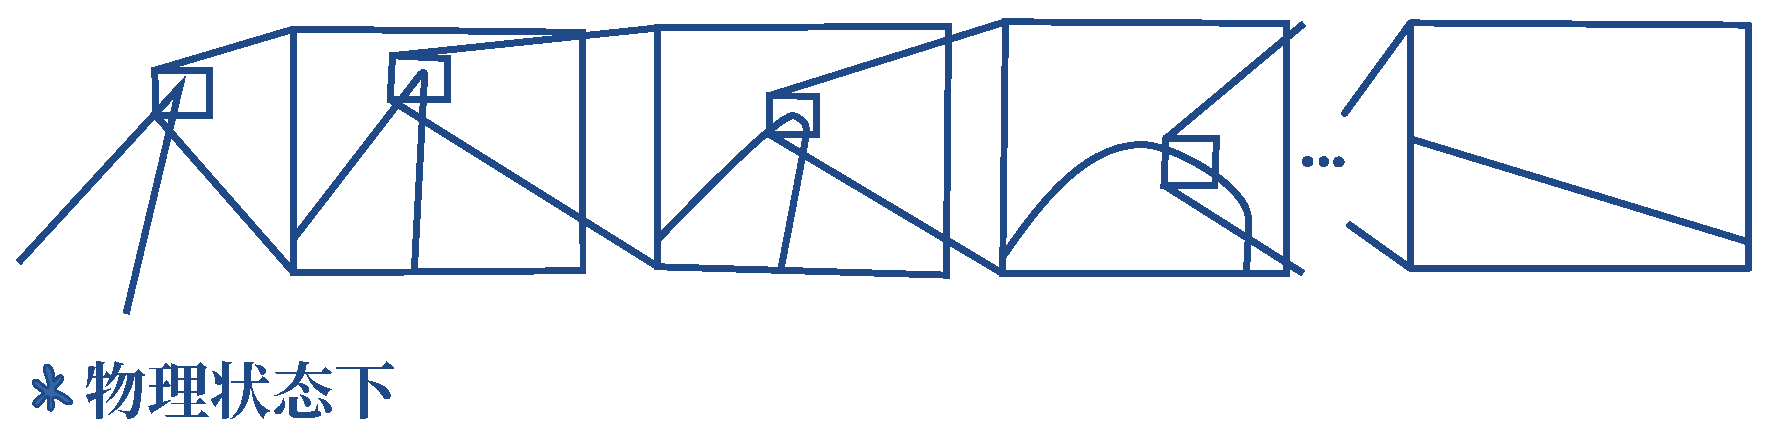
\includegraphics[scale=0.3]{PIC/003.eps}
					\caption{极限是光滑的}
					\label{Pic::极限是光滑的}
				\end{figure}

				比如说,汽车的速度计不能显示车辆运行的方向,所以,它显示的是汽车的瞬时速率,数值上也等于瞬时速度的大小.

			\subsubsection{例题}
				\paragraph{1}(\emph{苏州市高三期初调研,多选})
					两个物体$A$,$B$的加速度$a_A>a_B$,则\mathcnl\\
					A. $A$的速度一定比$B$的速度大.\\
					B. $A$的速度变化量一定比$B$的速度变化量大.\\
					C. $A$的速度变化一定比$B$的速度变换快.\\
					D. $A$的速度变换率一定比$B$的速度变化率大.\\
				\paragraph{2}(\emph{宿迁市高三模拟})
					\begin{figure}
						\begin{center}
							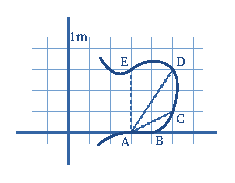
\includegraphics[scale=2]{PIC/004.eps}
							\caption{物体沿曲线轨迹的箭头方向运动}
							\label{Pic::物体沿曲线轨迹的箭头方向运动}
						\end{center}
					\end{figure}
					如图\ref{Pic::物体沿曲线轨迹的箭头方向运动}所示,物体沿曲线轨迹的箭头方向运动,$AB$、$ABC$、$ABCD$、$ABCDE$四段曲线%
					轨迹运动所用的时间分别是$1s$、$2s$、$3s$、$4s$,则下列说法\emph{错误}的是%
					\mathc\\
					A. 物体在$AB$段的平均速度为$1m/s$.\\
					B. 物体在$ABC$段的平均速度为$\frac{\sqrt{5}}{2}m/s$.\\
					C. $AB$段的平均速度比$ABC$段的平均速度更能反映出$A$点时的瞬时速度.\\
					D. 物体在$B$点的速度等于$AC$段的平均速度.\\
				\paragraph{3}
							汽车从甲城以速度$v_1$沿直线一直行驶到乙城,紧接着又从乙城以速度%
							$v_2$沿直线返回,到达甲、乙两城中点的丙小镇,关于汽车在这一全过程%
							中的平均速度,下列说法正确的是\mathc\\
							A. $\frac{v_1+v_2}{2}$,方向为甲指向丙.
							B. $\frac{v_1+v_2}{2}$,方向为乙指向丙.
							C. $\frac{v_1v_2}{v_1+2v_2}$,方向为乙指向丙.
							D. $\frac{v_1v_2}{v_1+2v_2}$,方向为甲指向丙.
				\paragraph{4}(\emph{盐城市高三联考})
					一辆汽车在一条平直公路上行驶,先以$108km/h$的速度行驶全程的%
					$\frac{1}{4}$,接着以$36km/h$的速度行驶完其余的$\frac{3}{4}$,%
					求汽车在全程内的平均速度大小.


		\subsection{实验:用打点计时器测速度}
			\subsubsection*{两种打点计时器}
				\paragraph{电磁打点计时器}
					电磁打点器的工作电压和工作频率是多少?它的工作原理又是什么呢?
				\paragraph{电火花计时器}
					电火花计时器在什么电压下工作呢?它是通过什么来工作的?

			\subsubsection*{打点计时器的原理}
				\paragraph{}理想情况下,打点计时器的打点时长可以看作为零\footnote{当然,实际上打点时长一定不为零,只是因为打点计时器的工作原理,所以打点计时器的打点时长很短,可以说是接近于零。在理想情况下看做零,就可以把打点计时器留下来的印记看做是一个点了},所以会在纸带上留下很多点的痕迹。因为它们的工作频率,它们会每隔$0.02s$打出一个点,两点之间就是纸带在该时间(\emph{即$0.02s$内})内走过的位移的大小。

			\subsubsection*{用打点计时器测量瞬时速度}
				又瞬时速度的定义可知,只有当$t\to 0$的时候下的平均速度才是瞬时速度。可是这在现实生活中难以实现,但是在一些情况下根据理论也可以求出理论下的瞬时速度。

				比如在图\ref{Pic::纸带和点}中,使用$D$,$F$两点的距离除以$0.06 s$(\emph{$D$、$F$之间有三个由点分开的距离,根据打点计时器的工作频率,容易知道,它们之间的距离对应的时间是$0.02 s\times 3=0.06s$})就可以算出$DF$的平均速度。而$D$、$F$的平均速度的大小,就和$E$的瞬时速度相近了。

				我们知道,距离越短,时间相应越小,而所求的平均速度就越等于所求点的瞬时速度。

				那么理论上的瞬时速度到底该怎么求呢?它到底需要满足什么条件呢?它和其他的点构成的路程和所对应的时间到底有什么联系呢?
				\begin{figure}
					\begin{center}
						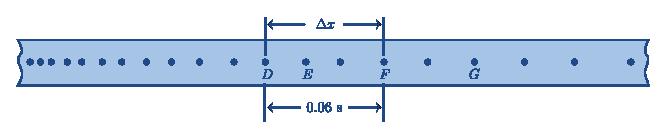
\includegraphics[]{PIC/005.eps}
						\caption{纸带和点}
						\label{Pic::纸带和点}
					\end{center}
				\end{figure}

			\subsubsection*{用图像来表示速度}
				如图\ref{Pic::打点计时器的速度-时间图像}所示,将手拉纸带的原始数据处理后就得到了一个$v-t$图像。在处理之后,图\ref{Pic::打点计时器的速度-时间图像}的丙图就是最接近现实情况的图像。\footnote{Q: 为什么要处理成丙图的样子?为什么不建议使用乙图呢?}

				使用$v-t$图像,可以直观地了解到物体的运动情况。
				\begin{figure}[!h]
					\begin{center}
						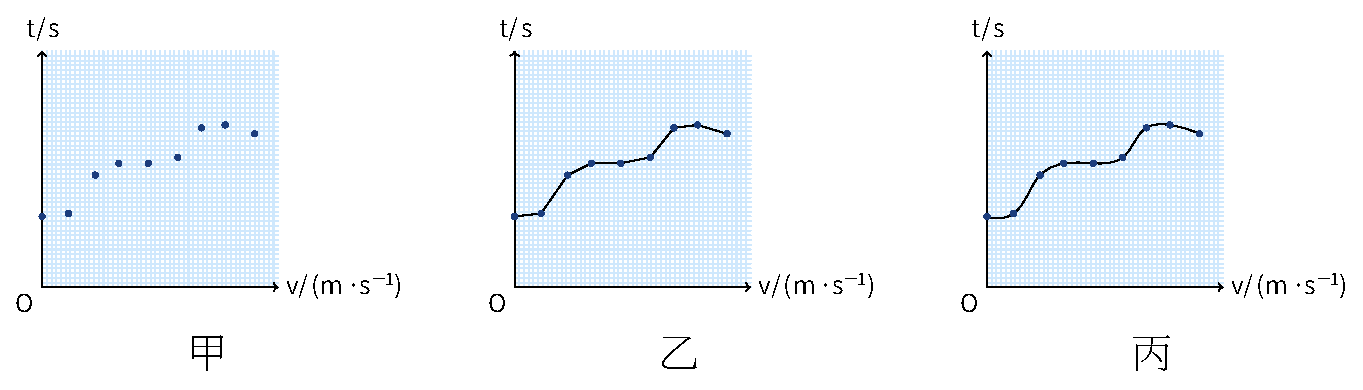
\includegraphics[scale=0.5]{PIC/006.eps}
						\caption{打点计时器的速度-时间图像}
						\label{Pic::打点计时器的速度-时间图像}
					\end{center}
				\end{figure}

			\subsection{速度变化快慢的描述 ----- 加速度}
				小汽车和列车都可以达到$100 km/h$,但是它们到达这样的速度所用的时间是不一样的,我们直观地感受到小轿车起步$20s$后速度就已经达到了$100 km/h$,但是火车却需要$500 s$,\emph{速度大}、\emph{速度变化大}和\emph{速度变化得快}是三种不同的情况。
				
				\subsubsection*{加速度}
					加速度是速度的变化量与发生这一变化过程所用时间的比值。通常用$a$来表示。

					若用$\Delta v$表示速度在时间间隔$\Delta t$内发生的变化,则有:
						$$a=\frac{\Delta v}{\Delta t}$$
					在国际单位制里面,加速度的单位是\emph{米每二次方秒},符号是$m/s^2$或$m\cdot s^{-2}$。

				\subsubsection*{加速度方向与速度方向的关系}
					加速度和速度是紧密联系在一起的,但是它们在一个瞬间并不能相互决定。

					比如说:
					\begin{itemize}
						\item 有可能出现速度大,但是加速度小的情况吗?
						\item 有可能出现速度变化量小,而加速度大的情况吗?
						\item 有可能出现速度方向与加速度方向相反的情况吗?
						\item 有可能出现加速度方向与速度变化量相反的情况吗?
						\item 有可能出现加速度增加而速度减少的情况吗?
						\item 物体速度为零,那么它的加速度一定为零吗?
					\end{itemize}

					可以看出,企图简单的考虑加速度和速度之间的关系是显得比较冒昧的。%
					考虑加速度和速度之间的关系时,必须要用速度变化量作为中间桥梁。%
					所以说,加速度大,速度变化快(\emph{在单位时间内变化量大}),在下一单位时间内速度会发生较大的变化。%
					所以说,速度大,加速度不一定大;加速度大,速度也不一定大。

					加速度和速度变化量一样(\emph{因为是由它推导出来的物理量}),是矢量。%
					它的方向\footnote{无论如何,在研究矢量的时候一定要注意到矢量的方向性。同学们一般都会过重看待矢量的大小而不注意它的方向性。但同时又要注意的是,方向和大小是独立的,方向也不会改变矢量的大小。比如定义在一维数轴上的速度$v_1$和$v_2$,满足$v_1=5m/s$,而$v_2=-7m/s$,虽然$v_2$定义下的值是负数,但是$v_2$是向量,向量的大小不可能为零(\emph{两点之间的距离不可能为零}),它的大小是它的绝对值,即$7m/s$,所以$v_2$的大小大于$v_1$,那么,值旁边的负数符号到底代表了什么意思呢?}在决定物体运动的性质上也有重要作用:
					\begin{enumerate}
						\item 加速运动$\to$加速度与速度同向
						\item 减速运动$\to$加速度与速度反向
					\end{enumerate}

					根据图\ref{Pic::速度-时间图像示意}中,解答以下问题:
					\begin{enumc}
						\item 如何表示加速度的大小\footnote{要记住加速度的定义呀。}?
						\item 物体做直线运动的加速度变化吗?为什么?
						\item $a$、$b$两个物体加速度的大小关系是怎么样的呢?
					\end{enumc}
					\begin{figure}
						\begin{center}
							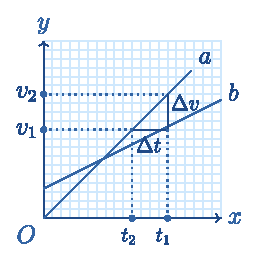
\includegraphics[]{PIC/007.eps}
							\caption{速度-时间图像示意}
							\label{Pic::速度-时间图像示意}
						\end{center}
					\end{figure}

					当然,运动也不止在一维平面发生,那么,在二维平面上,物体的速度大小未发生变化,那么其加速度的大小一定为零吗?

				\subsubsection{例题}
					\paragraph{1}比较速度与加速度的物理意义,判断下列说法是否正确,举例说明你的理由。其中正确的是\mathc\\
					A. 加速度不为零的运动速度一定增加.\\
					B. 两物体相比,一个物体的速度变化量比较大,加速度一定大.\\
					C. 物体运动越来越快,其加速度一定越来越大.\\
					D. 物体速度变化越来越慢,物体的加速度越来越小.\\
					E. 相等时间内速度变化大的物体,加速度大.\\

					\paragraph{2}对下列物理公式的理解,说法正确的是\mathc\\
					A. 由公式$a=\frac{\Delta v}{t}$可知,加速度$a$由速度的变化量$\Delta v$和时间$t$决定.\\
					B. 速度方向改变,加速度方向一定改变.\\
					C. 加速度大的物体运动得快.\\
					D. 加速度不为零时速度一定改变.\\


\end{document}
